De business laag is de plek waar de communicatie met de datalaag en de service laag plaats vindt. Vanwege de keuze om de data realtime door te geven aan de applicatie is het belangrijk dat deze laag snel en vloeiend werkt, ook bij een hoge load. Om deze reden hebben we gekozen voor een Cloud oplossing in Windows Azure, welke draait op een of meerdere cloud instances. Bij een hogere load worden er automatisch meerdere instances bij aangemaakt en wordt de load evenwichtig verdeeld. Tevens biedt een Cloud oplossing de mogelijkheid om verbeteringen aan bestaande of juist nieuwe functionaliteit toe te voegen aan de back-end, zonder dat hierbij de applicatie een update vereist.

Hoewel er meerdere soortgelijke cloud oplossingen bestaan, ging door de bestaande infrastructuur van Emando de voorkeur uit naar Windows Azure. Daarnaast integreert Windows Azure eenvoudig met Visual Studio, waardoor het deployen naar de cloud- of test-omgeving gemakkelijk kon.

\subsection{Aggregatie structuur}
Omdat de ruwe doorkomsten niet direct betekenis hebben voor gebruikers, dient deze data verrijkt te worden om zo inzicht te geven in trainingen van gebruikers. Dit proces noemen we de aggregatie van data.

\begin{wrapfigure}{r}{0.4\textwidth}
  \begin{center}
    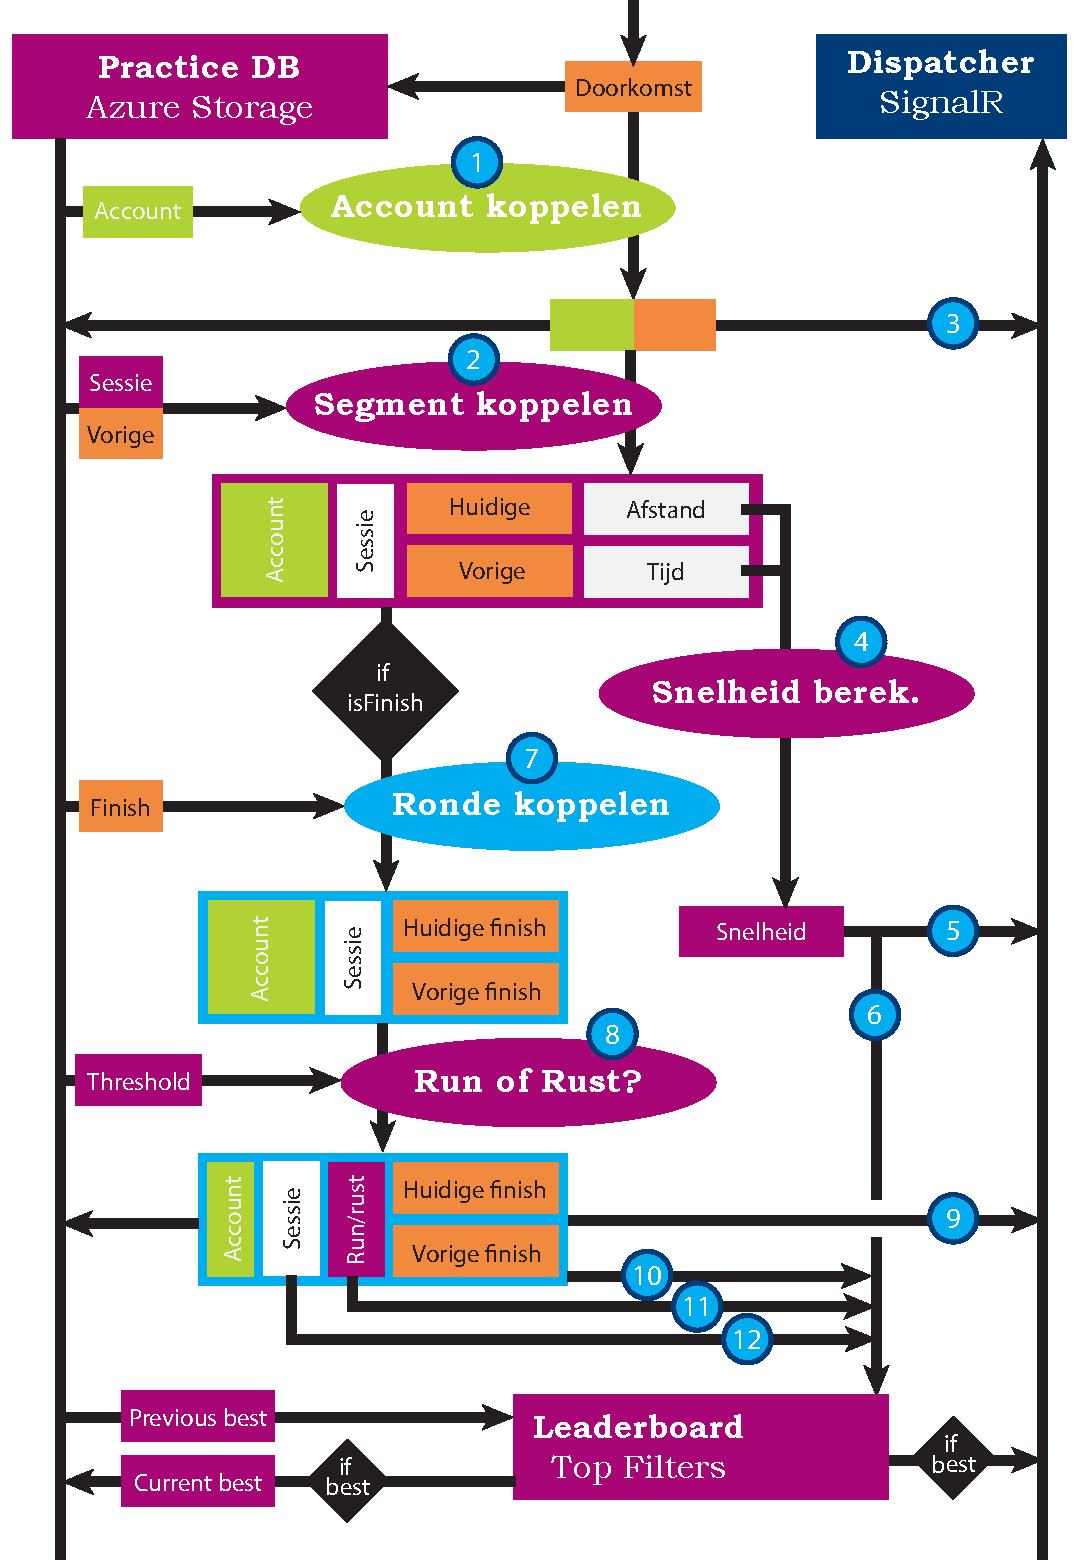
\includegraphics[width=.4\textwidth]{style/images/Aggregatie-flow}
  \end{center}
  \caption{Flow-diagram van het aggregatie process \\ deze afbeelding is in groot formaat opgenomen in Appendix~\ref{ch:aggregation-flow} op pagina~\pageref{fig:aggregatie-flow-large}}
  \label{fig:aggregatie-flow}
\end{wrapfigure}

Zodra er een doorkomst binnenkomt binnen de data laag, wordt het Id hiervan naar de aggregatie laag overgestuurd via de Azure Service Bus. Zodra de aggregatie laag deze ontvangt, wordt de bijbehorende doorkomst opgevraagd. Hierna start het aggregatie proces, dat bestaat uit de volgende onderdelen, zoals ook te zien is in figuur~\ref{fig:aggregatie-flow}:

\begin{itemize}
\item \textbf{Reguliere filters.}
Deze filters vergelijken reeds bestaande geaggregeerde en ruwe data met de nieuwste binnenkomst, om zo nieuwe data te aggregeren. Deze data wordt vervolgens doorgegeven aan de dispatchers en top filters. Voorbeeld: Het opmaken van rondetijden aan de hand van verschillende doorkomsten op een baan.
\item \textbf{Top filters.}
Deze filters vergelijken reeds bestaande geaggregeerde data met de zojuist geaggregeerde data, om zo te kijken of de zojuist geaggregeerde data een record bevat voor de gebruiker. Deze filters verwerken de nieuwe records in de leaderboards voor een gebruiker op gebruiker-, baan- en groep-niveau. Vervolgens worden deze leaderboards doorgegeven aan de dispatchers. Voorbeeld: Een gebruiker heeft een nieuwe ronde geschaatst, waarin zijn rondetijd verbeterd is. Ook is zijn totale afstand op de baan veranderd. 
\item \textbf{Dispatchers.}
De dispatchers ontvangen alle geaggregeerde data en zijn verantwoordelijk voor het doorgeven van deze data aan de juiste applicaties. De dispatchers zorgen er voor dat deze data realtime binnen komt bij alle geïnteresseerden van deze updates. 
Voorbeeld: Live doorkomsten van gebruikers van een groep/baan. 
\end{itemize}

De filters zijn opgebouwd volgens een pijpleiding structuur een filter geen aggregatie uit kan voeren, stopt de vertakking van aggregaties. De overige filters die hier van gebruik maken, kunnen immers niet aggregeren zonder de aggregatie uit de vorige pijpleiding.

\begin{enumerate}

\item \textbf{Account koppelen aan doorkomsten.}
Allereerst wordt bij een doorkomst aan de hand van het transponder nummer een account gezocht. Als er een bestaande gebruiker is die dit transponder nummer momenteel aan zijn account gekoppeld heeft, wordt dit account gekoppeld aan deze doorkomst. Dit wordt opgeslagen in een aparte tabel in Azure Table Storage.

\item \textbf{Doorkomsten koppelen aan segmenten.}
Een doorkomst maakt deel uit van een training, soms gekoppeld aan een trainingsschema. Deze kunnen bestaan uit een of meerdere sessies. (zie begrippenlijst). Een segment van doorkomsten houdt in dat er 2 doorkomsten van dezelfde gebruiker binnen 30 minuten plaatst hebben gevonden op dezelfde baan. Wanneer de vorige doorkomst van deze gebruiker en de huidige doorkomst binnen een segment vallen, vallen deze doorkomsten onder dezeflde trainingssessie. Wanneer dit het geval is, krijgt de doorkomst dezelfde sessie Id toegewezen als zijn vorige doorkomst. Wanneer dit niet het geval is of er geen vorige doorkomst is, kan er geen segment gevonden worden.

\item \textbf{Dispatchen van live doorkomsten.}
Zodra er een gebruiker gevonden is bij een doorkomst, moet deze doorgegeven worden aan alle geinteresseerden: mensen op dezelfde baan, mensen in dezelfde groep als deze gebruiker, de gebruiker zelf en alle mensen die geabbonneert zijn op deze gebruiker.

Met behulp van SignalR wordt de doorkomst doorgegeven aan de juiste personen.

\item \textbf{Snelheid berekenen.}
Tussen twee doorkomsten in een segment ligt een bepaalde afstand. Een gebruiker heeft deze afstand afgelegd in een tijdsinterval. Aan de hand van deze gegevens wordt de snelheid binnen dit segment berekend.

\item \textbf{Dispatchen van snelheden.}
Zodra er een snelheid is berekend voor een gebruiker op een bepaald segment, moet deze doorgegeven worden aan alle geïnteresseerden: mensen op dezelfde baan, mensen in dezelfde groep als deze gebruiker, de gebruiker zelf en alle mensen die geabbonneert zijn op deze gebruiker.

Met behulp van SignalR wordt de doorkomst doorgegeven aan de juiste personen.

\item \textbf{Snelheid leaderboard updaten en dispatchen.}
Zodra er een snelheid is berekend kan worden over een bepaald segment, kan dit gevolgen hebben voor het snelheids leaderboard. De gereden snelheid wordt vergeleken met de records voor een gebruiker van zijn eigen totale records, zijn records op deze baan en zijn records in al zijn groepen. Daarnaast wordt altijd de gereden afstand op de baan, tijdsinterval etc. bijgewerkt in de totalen binnen dit leaderboard. Wanneer de zojuist gereden snelheid een record blijkt te zijn voor een van zojuist genoemde contexten, wordt deze up to date gebracht in de leaderboards. Daarna wordt het gehele leaderboard voor deze context naar alle geïnteresseerden toegestuurd via SignalR.

\item \textbf{Doorkomsten koppelen aan rondes.}
De gevonden sessie bij het segment kan gebruikt worden om rondes te vinden. Zodra de vorige doorkomst van een gebruiker die op de finishlijn ligt het zelfde sessie Id heeft als de huidige doorkomst en de huidige doorkomst in het segment ook op de finish lijnligt, is er sprake van een ronde in een training. 
Wanneer het sessie Ids niet overeenkomen, of de huidige doorkomst niet op de finish lijn ligt is het niet mogelijk om een ronde te vinden.

\item \textbf{Filteren van run/rust rondes.}
Afhankelijk van het type sporter, wordt er soms getraind aan de hand van een trainingsschema. Deze schema's bestaan vaak uit rust en run periodes waarin respectievelijk rustig en hard getraind wordt. Omdat de lengte van rondes kan variëren op verschillende banen, wordt niet aan de hand van tijden, maar snelheden gefilterd. Wanneer een gebruiker een gemiddelde snelheid over zijn ronde hoger dan zijn zelf ingestelde snelheid om te filteren heeft ingesteld, wordt deze ronde beschouwd als een run ronde. Anders wordt deze beschouwd als een rust periode. Nu alle ronde data compleet is, wordt deze ronde opgeslagen in een aparte tabel in Azure Table Storage voor latere aggregaties.

\item \textbf{Dispatchen van rondes.}
Zodra er een ronde is berekend voor een gebruiker, moet deze doorgegeven worden aan alle geïnteresseerden: mensen op dezelfde baan, mensen in dezelfde groep als deze gebruiker, de gebruiker zelf en alle mensen die geabbonneert zijn op deze gebruiker.

Met behulp van SignalR wordt de doorkomst doorgegeven aan de juiste personen.

\item \textbf{Ronde leaderboard updaten en dispatchen.}
Zodra er een ronde is gevonden voor een gebruiker, kan dit gevolgen hebben voor het ronde leaderboard. De gereden ronde wordt vergeleken met de records voor een gebruiker van zijn eigen totale records, zijn records op deze baan en zijn records in al zijn groepen. Daarnaast wordt altijd de gereden afstand op de baan, tijdsinterval etc. bijgewerkt in de totalen binnen dit leaderboard. Wanneer de zojuist gereden rondetijd een record blijkt te zijn voor een van zojuist genoemde contexten, wordt deze up to date gebracht in de leaderboards. Daarna wordt het gehele leaderboard voor deze context naar alle geïnteresseerden toegestuurd via SignalR.

\item \textbf{Run/rust leaderboard updaten en dispatchen.}
Zodra er een ronde is gevonden voor een gebruiker, kan dit gevolgen hebben voor het run/rust leaderboard. De gereden rondetijd wordt toegevoegd aan de desbetreffende run/rust periode en aan de hand hiervan wordt het totaal hiervan vergeleken met de records voor een gebruiker van zijn eigen totale records, zijn records op deze baan en zijn records in al zijn groepen. Daarnaast wordt altijd de gereden afstand op de baan, tijdsinterval etc. bijgewerkt in de totalen binnen dit leaderboard. Wanneer de zojuist gereden rondetijd een record blijkt te zijn voor een van zojuist genoemde contexten, wordt deze up to date gebracht in de leaderboards. Daarna wordt het gehele leaderboard voor deze context naar alle geïnteresseerden toegestuurd via SignalR.

\item \textbf{Sessie leaderboard updaten en dispatchen.}
Zodra er een ronde is gevonden voor een gebruiker, kan dit gevolgen hebben voor het sessie leaderboard. De gereden rondetijd wordt toegevoegd aan de desbetreffendesessie en aan de hand hiervan wordt het totaal hiervan vergeleken met de records voor een gebruiker van zijn eigen totale records, zijn records op deze baan en zijn records in al zijn groepen. Daarnaast wordt altijd de gereden afstand op de baan, tijdsinterval etc. bijgewerkt in de totalen binnen dit leaderboard. Wanneer de zojuist gereden rondetijd een record blijkt te zijn voor een van zojuist genoemde contexten, wordt deze up to date gebracht in de leaderboards. Daarna wordt het gehele leaderboard voor deze context naar alle geïnteresseerden toegestuurd via SignalR.

\end{enumerate}

\subsection{Data consistentie en paralellisering}
Vanwege de meeschalende cloud oplossing, kan het voorkomen dat aggregaties van 1 persoon over meerdere instances berekend worden. Het is belangrijk dat deze aggregaties paralel lopen om gebruikers van realtime updates te kunnen voorzien. Dit brengt echter wel het probleem met zich mee dat sommige data afhankelijk is van andere data en dat deze data consistent moet blijven met elkaar. De bovengenoemde pijpleiding architectuur zorgt er voor dat bij ieder filter bekend is welke afhankelijkheden hierop berusten. Zodra het filter klaar is met zijn aggregatie, wordt gekeken of de aggregatie bruikbaar is voor zijn afhankelijkheden en geeft zijn aggregatie aan de hand hiervan door. Deze afhankelijkheden kunnen op hun beurt over verschillende instances verdeeld worden, zonder dat er opstoppingen ontstaan.

Omdat onze aggregatielaag berust op de MyLAPS SDK en een service bus, kan het in theorie voorkomen dat een eerdere doorkomst pas later bij deze laag binnenkomt dan een latere doorkomst. Ook kan het voorkomen dat het berekenen van een aggregatie van een eerdere doorkomst langer duurt dan die van een latere doorkomst, waardoor de updates hiervan door elkaar heen gaan lopen. Dit is te zien in figuur~\ref{fig:aggregatie-timing-problem}. 
In dit figuur is te zien hoe doorkomst 3 later gereden wordt, maar eerder geaggregeerd wordt dan doorkomst 2 welke eerder gereden is. Doordat de aggregatie werkt met de vorige doorkomst (doorkomst 1) wordt doorkomst 3 gekoppeld aan doorkomst 1 in een segment waarover de snelheid berekend wordt. Hieruit komt een correcte waarde.

Wanneer doorkomst 2 echter geaggregeerd wordt, vraagt deze de vorige doorkomst op. Omdat doorkomst 3 al geaggregeerd was is zijn vorige doorkomst 3. Hierbij wordt doorkomst 2 gekoppeld aan doorkomst 3. In dit segment blijkt nu -100 meter gereden te zijn. Er zou nu een verkeerde aggregatie ontstaan!

Daarom is het belangrijk dat de data ten alle tijden consistent is, ook over meerdere cloud instances.
Om deze reden zijn alle repositories calls voorzien van een synchronisatie tijdstip. Dit is het tijdstip waarop de doorkomst doorgekomen is. Deze calls geven daarmee alleen (aggregatie)-data terug die op het moment van de doorkomst beschikbaar was. In het bovengenoemde geval zou doorkomst 2 daarom óók gekoppeld worden aan doorkomst 1, vanwege het feit dat doorkomst 3 later binnen gekomen is dan doorkomst 2. Op deze manier worden inconsistenties in de data voorkomen.

\begin{figure}[ht]
  \begin{center}
    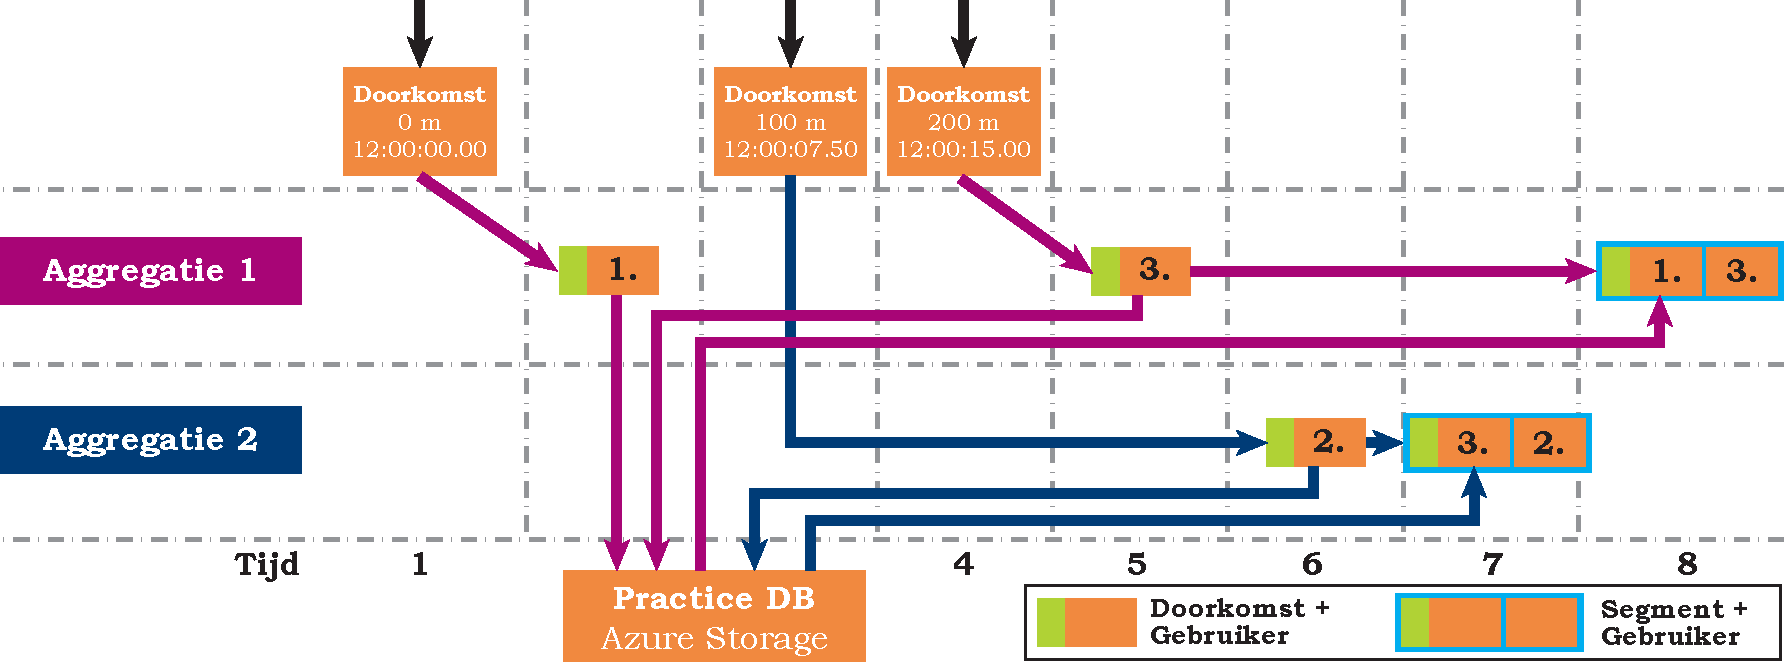
\includegraphics[width=\textwidth]{style/images/aggregatie-timing-problem}
  \end{center}
  \caption{Flow-diagram van hoe de data stroom verkeerd kan gaan.}
  \label{fig:aggregatie-timing-problem}
\end{figure}

Voor de leaderboards is gekozen om deze te verspreiden over 4 aparte tabellen. Leaderboards bestaan uit data die vanuit verschillende filters aangepast worden. Hierbij wordt eerst het leaderboard opgevraagd en daarna de update teruggeschreven naar de tabel. Bij het updaten is het mogelijk om een merge-operatie uit te voeren, waarbij alleen de beschikbare data (bijvoorbeeld een snelheid leaderboard) bij te werken zonder daarbij de bestaande data aan te passen. Dit kan echter alleen wanneer de ETag eigenschap van dit leaderboard ondertussen niet gewijzigd is. Deze eigenschap is een eigenschap van Azure Table Storage, die bijhoudt of het record in de tussentijd niet gewijzigd is. In de praktijk komt dit vaak voor, omdat er meerdere filters paralel aan elkaar dit record bij proberen te werken voor andere leaderboard eigenschappen. Om deze reden is beter om deze leaderboard te spreiden over meerdere tabellen.

